\chapter{Graph}
\section{Thinking in Graphs}
Since graphs are very common in daily life, we should be able to translate real-world problems into graph-related terms.

\subsubsection*{Takeaway}
When designing a BFS algorithm, you should:
\begin{itemize}
\item Carefully check the neighboring nodes, only enqueue those that are valid for exploration.
\item For any conditions or states influencing the decision to explore a neighboring node, update these states as soon as possible.
\end{itemize}

\section{LC 0133 - Clone Graph}\label{lc0133}
Given a pointer of a node in a {\color{blue}{connected undirected graph}}, return a {\color{blue}{deep copy}} of the graph. \\

The definition of {\colorbox{CodeBackground}{\lstinline|Node|}} is as follows.
\begin{lstlisting}
class Node {
 public:
	Node() {
		val = 0;
		neighbors = std::vector<Node*>();
	}
	Node(int _val) {
		val = _val;
		neighbors = std::vector<Node*>();
	}
	Node(int _val, std::vector<Node*> _neighbors) {
		val = _val;
		neighbors = _neighbors;
	}
	
	int val;
	std::vector<Node*> neighbors;
};
\end{lstlisting}

\subsection*{Analysis}
We cannot borrow algorithms from
\hyperref[chap:graph_boilerplate]{Chapter \ref{chap:graph_boilerplate}} directly because deep copy of a node can only be done after all its neighbors are traversed. This means the visit of current node are mixed up with further visit of its neighbors.

\subsection*{Solution 1 - BFS}
\begin{lstlisting}
	Node* cloneGraph(Node* node) {
		if (!node) { return nullptr; }
		std::queue<Node*> q;
		std::unordered_map<Node*, Node*> origin2copy;
		q.push(node);
		// shallow copy
		origin2copy[node] = new Node(node->val);
		while (!q.empty()) {
			Node* front = q.front();
			q.pop();
			for (auto& neighbor : front->neighbors) {
				if (origin2copy.find(neighbor) == origin2copy.end()) {
					origin2copy[neighbor] = new Node(neighbor->val);
					q.push(neighbor);
				}
				// deep copy can only be done after all its neighbors are traversed
				origin2copy[front]->neighbors.push_back(origin2copy[neighbor]);
			}
		}
		return origin2copy[node];
	}
\end{lstlisting}

\subsection*{Solution 2 - DFS}
\begin{lstlisting}
Node* cloneGraph(Node* node) {
	std::unordered_map<Node*, Node*> origin2copy;
	return cloneGraph(node, origin2copy);
}

Node* cloneGraph(Node* node, std::unordered_map<Node*, Node*>& origin2copy) {
	if (!node) { return nullptr; }
	if (origin2copy.find(node) == origin2copy.end()) {
		// shallow copy
		origin2copy[node] = new Node(node->val);
		for (auto& neighbor : node->neighbors) {
			// deep copy can only be done after all its neighbors are traversed
			origin2copy[node]->neighbors.push_back(cloneGraph(neighbor, origin2copy));
		}
	}
	return origin2copy[node];
}
\end{lstlisting}

\subsection*{Solution 3 - DFS with {\colorbox{CodeBackground}{\lstinline|static|}} Variable}
\begin{lstlisting}
Node* cloneGraph(Node* node) {
	if (!node) { return nullptr; }
	static std::unordered_map<Node*, Node*> origin2copy;
	if (origin2copy.find(node) == origin2copy.end()) {
		// shallow copy
		origin2copy[node] = new Node(node->val);
		for (auto& neighbor : node->neighbors) {
			// deep copy can only be done after all its neighbors are traversed
			origin2copy[node]->neighbors.push_back(cloneGraph(neighbor));
		}
	}
	return origin2copy[node];
}
\end{lstlisting}

\subsection*{Related}
\begin{itemize}
	\item \hyperref[lc0138]{LC 0138 - Copy List with Random Pointer}
	\item \hyperref[lc0133]{LC 0133 - Clone Graph}
\end{itemize}

\section{LC 0127 - Word Ladder}
A transformation sequence from word {\colorbox{CodeBackground}{\lstinline|beginWord|}} to word {\colorbox{CodeBackground}{\lstinline|endWord|}} ({\colorbox{CodeBackground}{\lstinline|beginWord != endWord|}}) using a dictionary {\colorbox{CodeBackground}{\lstinline|wordList|}} is a sequence of words {\colorbox{CodeBackground}{\lstinline|beginWord|}}$\rightarrow${\colorbox{CodeBackground}{\lstinline|s1|}}$\rightarrow${\colorbox{CodeBackground}{\lstinline|s2|}}$\rightarrow${\colorbox{CodeBackground}{\lstinline|s3|}}$\dots\rightarrow\dots${\colorbox{CodeBackground}{\lstinline|sk|}} such that:
\begin{itemize}
	\item Every adjacent pair of words differs by a single letter.
	\item Every {\colorbox{CodeBackground}{\lstinline|s_i|}} for {\colorbox{CodeBackground}{\lstinline|1 <= i <= k|}} is in {\colorbox{CodeBackground}{\lstinline|wordList|}}. Note that {\colorbox{CodeBackground}{\lstinline|beginWord|}} does not need to be in {\colorbox{CodeBackground}{\lstinline|wordList|}}.
	\item {\colorbox{CodeBackground}{\lstinline|s_k == endWord|}}
\end{itemize}
Given two words, {\colorbox{CodeBackground}{\lstinline|beginWord|}} and {\colorbox{CodeBackground}{\lstinline|endWord|}}, and a dictionary {\colorbox{CodeBackground}{\lstinline|wordList|}}, return the number of words in the shortest transformation sequence from {\colorbox{CodeBackground}{\lstinline|beginWord|}} to {\colorbox{CodeBackground}{\lstinline|endWord|}}, or {\colorbox{CodeBackground}{\lstinline|0|}} if no such sequence exists.\\

Examples:
\begin{itemize}
	\item {\colorbox{CodeBackground}{\lstinline|beginWord = "hit", endWord = "cog", wordList = ["hot","dot","dog","lot","log","cog"] --> 5|}}
	\item {\colorbox{CodeBackground}{\lstinline|beginWord = "hit", endWord = "cog", wordList = ["hot","dot","dog","lot","log"] --> 0|}}
\end{itemize}

\subsection*{Translate into Graph Problem}

\subsection*{Solution}

\section{LC 0126 - Word Ladder II}
A transformation sequence from word {\colorbox{CodeBackground}{\lstinline|beginWord|}} to word {\colorbox{CodeBackground}{\lstinline|endWord|}} using a dictionary {\colorbox{CodeBackground}{\lstinline|wordList|}} is a sequence of words {\colorbox{CodeBackground}{\lstinline|beginWord|}}$\rightarrow${\colorbox{CodeBackground}{\lstinline|s1|}}$\rightarrow${\colorbox{CodeBackground}{\lstinline|s2|}}$\rightarrow${\colorbox{CodeBackground}{\lstinline|s3|}}$\dots\rightarrow\dots${\colorbox{CodeBackground}{\lstinline|sk|}} such that:
\begin{itemize}
	\item Every adjacent pair of words differs by a single letter.
	\item Every {\colorbox{CodeBackground}{\lstinline|s_i|}} for {\colorbox{CodeBackground}{\lstinline|1 <= i <= k|}} is in {\colorbox{CodeBackground}{\lstinline|wordList|}}. Note that {\colorbox{CodeBackground}{\lstinline|beginWord|}} does not need to be in {\colorbox{CodeBackground}{\lstinline|wordList|}}.
	\item {\colorbox{CodeBackground}{\lstinline|s_k == endWord|}}
\end{itemize}
Given two words, {\colorbox{CodeBackground}{\lstinline|beginWord|}} and {\colorbox{CodeBackground}{\lstinline|endWord|}}, and a dictionary {\colorbox{CodeBackground}{\lstinline|wordList|}}, return all the shortest transformation sequences from {\colorbox{CodeBackground}{\lstinline|beginWord|}} to {\colorbox{CodeBackground}{\lstinline|endWord|}}, or an empty list if no such sequence exists. Each sequence should be returned as a list of the words {\colorbox{CodeBackground}{\lstinline|[beginWord, s1, s2, ..., sk]|}}.

\subsection*{Translate into Graph Problem}

\subsection*{Solution}

\section{LC 0433 - Minimum Genetic Mutation}
A gene string can be represented by an 8-character long string, with choices from {\colorbox{CodeBackground}{\lstinline|'A'|}}, {\colorbox{CodeBackground}{\lstinline|'C'|}}, {\colorbox{CodeBackground}{\lstinline|'G'|}}, and {\colorbox{CodeBackground}{\lstinline|'T'|}}.\\

Suppose we need to investigate a \ul{mutation} from a gene string {\colorbox{CodeBackground}{\lstinline|startGene|}} to a gene string {\colorbox{CodeBackground}{\lstinline|endGene|}} where one mutation is defined as \ul{one single character changed} in the gene string. For example, {\colorbox{CodeBackground}{\lstinline|"AACCGGTT"|}} $\Rightarrow$ {\colorbox{CodeBackground}{\lstinline|"AACCGGTA"|}} is one mutation.\\

There is also a gene bank {\colorbox{CodeBackground}{\lstinline|bank|}} that records all the valid gene mutations. A gene must be in {\colorbox{CodeBackground}{\lstinline|bank|}} to make it a valid gene string.\\

Given the two gene strings {\colorbox{CodeBackground}{\lstinline|startGene|}} and {\colorbox{CodeBackground}{\lstinline|endGene|}} and the gene bank {\colorbox{CodeBackground}{\lstinline|bank|}}, return the minimum number of mutations needed to mutate from {\colorbox{CodeBackground}{\lstinline|startGene|}} to {\colorbox{CodeBackground}{\lstinline|endGene|}}. If there is no such a mutation, return {\colorbox{CodeBackground}{\lstinline|-1|}}.\\

Examples:
\begin{itemize}
	\item {\colorbox{CodeBackground}{\lstinline|startGene = "AACCGGTT", endGene = "AACCGGTA", bank = ["AACCGGTA"] --> 1|}}
	\item {\colorbox{CodeBackground}{\lstinline|startGene = "AACCGGTT", endGene = "AAACGGTA", bank = ["AACCGGTA","AACCGCTA","AAACGGTA"] --> 2|}}
\end{itemize}

\subsection*{Translate into Graph Problem}

\subsection*{Solution}

\section{LC 0399 - Evaluate Division}
You are given:
\begin{itemize}
	\item An array of variable pairs where {\colorbox{CodeBackground}{\lstinline|equations[i] = [A_i, B_i]|}}; Each {\colorbox{CodeBackground}{\lstinline|A_i|}} or {\colorbox{CodeBackground}{\lstinline|B_i|}} is a {\colorbox{CodeBackground}{\lstinline|std::string|}} that represents a single variable.
	\item An array of real numbers where {\colorbox{CodeBackground}{\lstinline|values[i] = A_i / B_i|}}. Note that {\colorbox{CodeBackground}{\lstinline|values.size() == equations.size()|}}.
	\item An array of queries where {\colorbox{CodeBackground}{\lstinline|queries[j] = [C_j, D_j]|}}, and you need to find the answer for {\colorbox{CodeBackground}{\lstinline|C_j / D_j = ?|}}
\end{itemize}

Return the answers to all queries. If a single answer cannot be determined, return {\colorbox{CodeBackground}{\lstinline|-1.0|}}.\\

It should be noted that the input is always valid. You may assume that evaluating the queries will not result in division by zero and that there is no contradiction.\\

Examples:
\begin{lstlisting}
// example 1
equations = [["a","b"],["b","c"]]
values = [2.0,3.0]
queries = [["a","c"],["b","a"],["a","e"],["a","a"],["x","x"]]
--> [6.00000,0.50000,-1.00000,1.00000,-1.00000]

// example 2
equations = [["a","b"],["b","c"],["bc","cd"]]
values = [1.5,2.5,5.0]
queries = [["a","c"],["c","b"],["bc","cd"],["cd","bc"]]
--> [3.75000,0.40000,5.00000,0.20000]

// example 3
equations = [["a","b"]]
values = [0.5]
queries = [["a","b"],["b","a"],["a","c"],["x","y"]]
--> [0.50000,2.00000,-1.00000,-1.00000]
\end{lstlisting}

\subsection*{Translate into Graph Problem}
We have some equations like {\colorbox{CodeBackground}{\lstinline|A / B = 2.0|}} and we need to answer queries like What is {\colorbox{CodeBackground}{\lstinline|A / C|}}?. The trick is to represent these equations as a graph where each {\color{blue}{variable}} is a {\color{blue}{node}} and the {\color{blue}{division}} is an {\color{blue}{edge}} with a {\color{blue}{weight}}. For example,{\colorbox{CodeBackground}{\lstinline| A / B = 2.0|}} means there's an edge from {\colorbox{CodeBackground}{\lstinline|A|}} to {\colorbox{CodeBackground}{\lstinline|B|}} with a weight of {\colorbox{CodeBackground}{\lstinline|2.0|}}, and an edge from {\colorbox{CodeBackground}{\lstinline|B|}} to {\colorbox{CodeBackground}{\lstinline|A|}} with a weight of {\colorbox{CodeBackground}{\lstinline|1/2.0|}}. To find {\colorbox{CodeBackground}{\lstinline|A / C|}}, we just need to find a path from {\colorbox{CodeBackground}{\lstinline|A|}} to {\colorbox{CodeBackground}{\lstinline|C|}} and multiply the weights of the edges along this path.

\subsection*{Solution - DFS}
The key part of this solution is the {\colorbox{CodeBackground}{\lstinline|AnswerQuery|}} function, which uses {\color{blue}{DFS}} to calculate the answer to a single query.
\begin{lstlisting}
class Solution {
 public:
	// create directed graph
	// node: variable, e.g., x, y
	// directed edge, e.g., x -> y is x / y
	void BuildGraph(std::vector<std::vector<std::string>>& equations, 
								  std::vector<double>& values) {
		for (int i = 0; i < equations.size(); ++i) {
			std::string x = equations[i][0];
			std::string y = equations[i][1];
			double val = values[i];
			graph[x][y] = val;
			graph[y][x] = 1.0 / val;
		}
	}
	
	// calculate answer for a single query
	double AnswerQuery(std::string start, std::string end, 
										  std::unordered_set<std::string>& visited) {
		if (start == end) { return 1.0; }
		visited.insert(start);
		for (auto& pair : graph[start]) {
			std::string next = pair.first;
			double value = pair.second;
			if (visited.find(next) == visited.end()) {
				double res = AnswerQuery(next, end, visited);
				if (res != -1.0) { return value * res; }
			}
		}
		return -1.0;
	}
	
	std::vector<double> calcEquation(std::vector<std::vector<std::string>>& equations,
	std::vector<double>& values,
	std::vector<std::vector<std::string>>& queries) {
		BuildGraph(equations, values);
		std::vector<double> answers;
		for (auto& query : queries) {
			std::string start = query[0];
			std::string end = query[1];
			if (graph.find(start) == graph.end() || graph.find(end) == graph.end()) {
				answers.push_back(-1.0);
			} else {
				std::unordered_set<std::string> visited;
				answers.push_back(AnswerQuery(start, end, visited));
			}
		}
		
		return answers;
	}
	
	std::unordered_map<std::string, std::unordered_map<std::string, double>> graph;
};
\end{lstlisting}

\section{LC 0207 - Course Schedule}\label{lc0207}
{\hyperref[sec:topological_sort]{[Topological Sort]}}\\

There are a total of {\colorbox{CodeBackground}{\lstinline|numCourses|}} ({\colorbox{CodeBackground}{\lstinline|numCourses >= 1|}}) courses you have to take, labeled from {\colorbox{CodeBackground}{\lstinline|0|}} to {\colorbox{CodeBackground}{\lstinline|numCourses - 1|}}.\\

You are given an array {\colorbox{CodeBackground}{\lstinline|prerequisites|}} where {\colorbox{CodeBackground}{\lstinline|prerequisites[i] = [a_i, b_i]|}} indicates that you must take course {\colorbox{CodeBackground}{\lstinline|b_i|}} first if you want to take course {\colorbox{CodeBackground}{\lstinline|a_i|}}.\\

Return {\colorbox{CodeBackground}{\lstinline|true|}} if you can finish all courses. Otherwise, return {\colorbox{CodeBackground}{\lstinline|false|}}.\\

Examples:
\begin{itemize}
\item {\colorbox{CodeBackground}{\lstinline|numCourses = 2, prerequisites = [[1,0]] --> true|}}
\item {\colorbox{CodeBackground}{\lstinline|numCourses = 2, prerequisites = [[1,0],[0,1]] --> false|}}
\end{itemize}

\subsection*{Solution}
Build a {\color{blue}{dependency graph}} and check if it is {\color{blue}{cyclic}}.

\begin{lstlisting}
bool DetectCycleFromNode(std::vector<std::vector<int>>& graph, int course,
												 std::vector<bool>& visited, std::vector<bool>& on_path) {
	if (course < 0 || course >= graph.size()) { return false; }
	if (on_path[course]) { return true; }
	if (visited[course]) { return false; }
	
	visited[course] = true;
	on_path[course] = true;
	for (int neighbor : graph[course]) {
		if (DetectCycleFromNode(graph, neighbor, visited, on_path)) { return true; }
	}
	on_path[course] = false;
	
	return false;
}

bool canFinish(int numCourses, std::vector<std::vector<int>>& prerequisites) {
	// build graph
	std::vector<std::vector<int>> graph(numCourses);
	for (const auto& pre : prerequisites) { graph[pre[1]].push_back(pre[0]); }
	
	// detect cycles
	std::vector<bool> visited(numCourses, false);
	std::vector<bool> on_path(numCourses, false);
	for (int i = 0; i < numCourses; ++i) {
		if (visited[i]) { continue; }
		if (DetectCycleFromNode(graph, i, visited, on_path)) { return false; }
	}
	
	return true;
}
\end{lstlisting}

\section{LC 0210 - Course Schedule II}\label{lc0210}
{\hyperref[sec:topological_sort]{[Topological Sort]}}\\

There are a total of {\colorbox{CodeBackground}{\lstinline|numCourses|}} ({\colorbox{CodeBackground}{\lstinline|numCourses >= 1|}} courses you have to take, labeled from {\colorbox{CodeBackground}{\lstinline|0|}} to {\colorbox{CodeBackground}{\lstinline|numCourses - 1|}}.\\

You are given an array {\colorbox{CodeBackground}{\lstinline|prerequisites|}} where {\colorbox{CodeBackground}{\lstinline|prerequisites[i] = [a_i, b_i]|}} indicates that you must take course {\colorbox{CodeBackground}{\lstinline|b_i|}} first if you want to take course {\colorbox{CodeBackground}{\lstinline|a_i|}}.\\

Return the ordering of courses you should take to finish all courses. If there are many valid answers, return any of them. If it is impossible to finish all courses, return an empty array.\\

Examples:
\begin{lstlisting}
// example 1
numCourses = 2, prerequisites = [[1,0]] --> [0,1]
// example 2
numCourses = 4, prerequisites = [[1,0],[2,0],[3,1],[3,2]] --> [0,2,1,3]
// example 3
numCourses = 1, prerequisites = [] --> [0]
\end{lstlisting}

\subsection*{Translate into Graph Problem}
Build a {\color{blue}{dependency graph}}, check if it is {\color{blue}{cyclic}}, and store the path.

\subsection*{Solution}
\begin{lstlisting}
bool DetectCycleFromNodeAndStorePath(const std::vector<std::vector<int>>& graph, int course,
																		 std::vector<bool>& visited, std::vector<bool>& on_path, 
																		 std::vector<int>& path) {
	if (course < 0 || course >= graph.size()) { return false; }
	if (on_path[course]) { return true; }
	if (visited[course]) { return false; }
	
	on_path[course] = true;
	visited[course] = true;
	for (int neighbor : graph[course]) {
		if (DetectCycleFromNodeAndStorePath(graph, neighbor, visited, on_path, path)) { 
			return true; 
		}
	}
	on_path[course] = false;
	
	path.push_back(course);
	
	return false;
}

std::vector<int> findOrder(int numCourses, std::vector<std::vector<int>>& prerequisites) {
	std::vector<std::vector<int>> graph(numCourses);
	for (const auto& p : prerequisites) { graph[p[1]].push_back(p[0]); }
	
	std::vector<bool> visited(numCourses, false);
	std::vector<bool> on_path(numCourses, false);
	std::vector<int> path;
	for (int i = 0; i < numCourses; ++i) {
		if (visited[i]) { continue; }
		// cycle detected
		if (DetectCycleFromNodeAndStorePath(graph, i, visited, on_path, path)) { return {}; }
	}
	// no cycle
	std::reverse(path.begin(), path.end());
	
	return path;
}
\end{lstlisting}

\section{LC 0630 - Course Schedule III}\label{lc0630}
{\hyperref[sec:topological_sort]{[Topological Sort]}}\\

There are {\colorbox{CodeBackground}{\lstinline|n|}} ({\colorbox{CodeBackground}{\lstinline|n >= 1|}}) different online courses numbered from {\colorbox{CodeBackground}{\lstinline|1|}} to {\colorbox{CodeBackground}{\lstinline|n|}}. You are given an array courses where {\colorbox{CodeBackground}{\lstinline|courses[i] = [duration_i, lastDay_i]|}} indicate that the {\colorbox{CodeBackground}{\lstinline|i|}}th course should be taken continuously for {\colorbox{CodeBackground}{\lstinline|duration_i|}} days and must be finished before or on {\colorbox{CodeBackground}{\lstinline|lastDay_i|}}.\\

You will start on the {\colorbox{CodeBackground}{\lstinline|1|}}st day and you cannot take two or more courses simultaneously.\\

Return the maximum number of courses that you can take.\\

Examples:
\begin{itemize}
\item {\colorbox{CodeBackground}{\lstinline|courses = [[100,200],[200,1300],[1000,1250],[2000,3200]] --> 3|}}
\item {\colorbox{CodeBackground}{\lstinline|courses = [[1,2]] --> 1|}}
\item {\colorbox{CodeBackground}{\lstinline|courses = [[3,2],[4,3]] --> 0|}}
\end{itemize}

\section{LC 1136 - Parallel Courses}\label{lc1136}
{\hyperref[sec:topological_sort]{[Topological Sort]}}\\

You are given an integer {\colorbox{CodeBackground}{\lstinline|n|}} ({\colorbox{CodeBackground}{\lstinline|n >= 1|}}), which indicates that there are {\colorbox{CodeBackground}{\lstinline|n|}} courses labeled from {\colorbox{CodeBackground}{\lstinline|1|}} to {\colorbox{CodeBackground}{\lstinline|n|}}. You are also given an array relations where {\colorbox{CodeBackground}{\lstinline|relations[i] = [prevCourse_i, nextCourse_i]|}}, representing a prerequisite relationship between course {\colorbox{CodeBackground}{\lstinline|prevCourse_i|}} and course {\colorbox{CodeBackground}{\lstinline|nextCourse_i|}}: course {\colorbox{CodeBackground}{\lstinline|prevCourse_i|}} has to be taken before course {\colorbox{CodeBackground}{\lstinline|nextCourse_i|}}.\\

In one semester, you can take any number of courses as long as you have taken all the prerequisites in the previous semester for the courses you are taking.\\

Return the minimum number of semesters needed to take all courses. If there is no way to take all the courses, return {\colorbox{CodeBackground}{\lstinline|-1|}}.

\begin{itemize}
\item Example 1: {\colorbox{CodeBackground}{\lstinline|n = 3, relations = [[1,3],[2,3]] --> 2|}}
\begin{figure}[H]
\centering
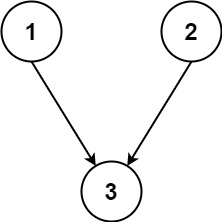
\includegraphics[width=0.15\linewidth]{images/lc1136_eg1}
\label{fig:lc1136eg1}
\end{figure}
\item Example 2: {\colorbox{CodeBackground}{\lstinline|n = 3, relations = [[1,2],[2,3],[3,1]] --> -1|}}
\begin{figure}[H]
\centering
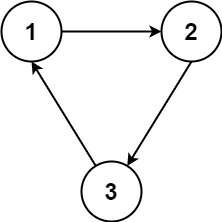
\includegraphics[width=0.15\linewidth]{images/lc1136_eg2}
\label{fig:lc1136eg2}
\end{figure}
\end{itemize}

\section{LC 1494 - Parallel Courses II}\label{lc1494}
{\hyperref[sec:topological_sort]{[Topological Sort]}}\\

You are given an integer {\colorbox{CodeBackground}{\lstinline|n|}} ({\colorbox{CodeBackground}{\lstinline|n >= 1|}}), which indicates that there are {\colorbox{CodeBackground}{\lstinline|n|}} courses labeled from {\colorbox{CodeBackground}{\lstinline|1|}} to {\colorbox{CodeBackground}{\lstinline|n|}}. You are also given an array relations where {\colorbox{CodeBackground}{\lstinline|relations[i] = [prevCourse_i, nextCourse_i]|}}, representing a prerequisite relationship between course {\colorbox{CodeBackground}{\lstinline|prevCourse_i|}} and course {\colorbox{CodeBackground}{\lstinline|nextCourse_i|}}: course {\colorbox{CodeBackground}{\lstinline|prevCourse_i|}} has to be taken before course {\colorbox{CodeBackground}{\lstinline|nextCourse_i|}}.\\

In one semester, you can take at most {\colorbox{CodeBackground}{\lstinline|k|}} ({\colorbox{CodeBackground}{\lstinline|k >= 1|}}) courses as long as you have taken all the prerequisites in the previous semesters for the courses you are taking.\\

Return the minimum number of semesters needed to take all courses.\\

Note: The test cases are generated such that it is possible to complete every course (i.e., the graph is a directed acyclic graph).

\begin{itemize}
\item {\colorbox{CodeBackground}{\lstinline|n = 4, relations = [[2,1],[3,1],[1,4]], k = 2 --> 3|}}
\begin{figure}[H]
\centering
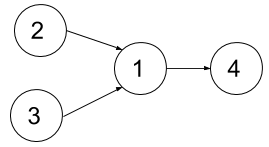
\includegraphics[width=0.3\linewidth]{images/lc1494_eg1}
\end{figure}
\item {\colorbox{CodeBackground}{\lstinline|n = 5, relations = [[2,1],[3,1],[4,1],[1,5]], k = 2 --> 4|}}
\begin{figure}[H]
\centering
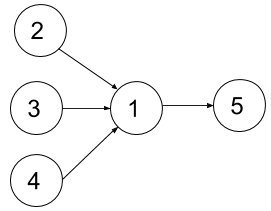
\includegraphics[width=0.3\linewidth]{images/lc1494_eg2}
\end{figure}
\end{itemize}

\section{LC 2050 - Parallel Courses III}\label{lc2050}
{\hyperref[sec:topological_sort]{[Topological Sort]}}\\

You are given an integer {\colorbox{CodeBackground}{\lstinline|n|}} ({\colorbox{CodeBackground}{\lstinline|n >= 1|}}), which indicates that there are {\colorbox{CodeBackground}{\lstinline|n|}} courses labeled from {\colorbox{CodeBackground}{\lstinline|1|}} to {\colorbox{CodeBackground}{\lstinline|n|}}. You are also given an array relations where {\colorbox{CodeBackground}{\lstinline|relations[i] = [prevCourse_i, nextCourse_i]|}}, representing a prerequisite relationship between course {\colorbox{CodeBackground}{\lstinline|prevCourse_i|}} and course {\colorbox{CodeBackground}{\lstinline|nextCourse_i|}}: course {\colorbox{CodeBackground}{\lstinline|prevCourse_i|}} has to be taken before course {\colorbox{CodeBackground}{\lstinline|nextCourse_i|}}.\\

Furthermore, you are given a {\colorbox{CodeBackground}{\lstinline|0|}}-indexed integer array {\colorbox{CodeBackground}{\lstinline|time|}} where {\colorbox{CodeBackground}{\lstinline|time[i]|}} denotes how many months it takes to complete the {\colorbox{CodeBackground}{\lstinline|(i+1)|}}th course.\\

You must find the minimum number of months needed to complete all the courses following these rules:
\begin{itemize}
\item You may start taking a course at any time if the prerequisites are met.
\item Any number of courses can be taken at the same time.
\end{itemize}

Return the minimum number of months needed to complete all the courses.\\

Note: The test cases are generated such that it is possible to complete every course (i.e., the graph is a directed acyclic graph).

\section{LC 0909 - Snakes and Ladders}
You are given an {\colorbox{CodeBackground}{\lstinline|n x n|}} integer matrix {\colorbox{CodeBackground}{\lstinline|board|}} where the cells are labeled from {\colorbox{CodeBackground}{\lstinline|1|}} to {\colorbox{CodeBackground}{\lstinline|n^2|}} in a \ul{Boustrophedon style} starting from the bottom left of the board (i.e. {\colorbox{CodeBackground}{\lstinline|board[n - 1][0]|}}) and alternating direction each row.\\

You start on square {\colorbox{CodeBackground}{\lstinline|1|}} of the board. In each move, starting from square {\colorbox{CodeBackground}{\lstinline|curr|}}, do the following:
\begin{itemize}
	\item Choose a destination square {\colorbox{CodeBackground}{\lstinline|next|}} with a label in the range {\colorbox{CodeBackground}{\lstinline|[curr + 1, min(curr + 6, n2)]|}}. This choice simulates the result of a standard {\colorbox{CodeBackground}{\lstinline|6|}}-sided die roll: i.e., there are at most {\colorbox{CodeBackground}{\lstinline|6|}} destinations, regardless of the size of the board.
	\item If {\colorbox{CodeBackground}{\lstinline|next|}} has a \ul{snake} or \ul{ladder}, you must move to the destination of that snake or ladder. Otherwise, you move to {\colorbox{CodeBackground}{\lstinline|next|}}. A board square on row {\colorbox{CodeBackground}{\lstinline|r|}} and column {\colorbox{CodeBackground}{\lstinline|c|}} has a snake or ladder if {\colorbox{CodeBackground}{\lstinline|board[r][c] != -1|}}. The destination of that snake or ladder is {\colorbox{CodeBackground}{\lstinline|board[r][c]|}}.
	\item The game ends when you reach the square {\colorbox{CodeBackground}{\lstinline|n^2|}}.
\end{itemize}

Note that:
\begin{itemize}
	\item  Squares {\colorbox{CodeBackground}{\lstinline|1|}} and {\colorbox{CodeBackground}{\lstinline|n^2|}} do not have a snake or ladder.
	\item You only take a snake or ladder at most once per move. If the destination to a snake or ladder is the start of another snake or ladder, you do not follow the subsequent snake or ladder.
\end{itemize}

Return the least number of moves required to reach the square {\colorbox{CodeBackground}{\lstinline|n^2|}}. If it is not possible to reach the square, return {\colorbox{CodeBackground}{\lstinline|-1|}}.\\

Example:
\begin{lstlisting}
board = [
[-1,-1,-1,-1,-1,-1],
[-1,-1,-1,-1,-1,-1],
[-1,-1,-1,-1,-1,-1],
[-1,35,-1,-1,13,-1],
[-1,-1,-1,-1,-1,-1],
[-1,15,-1,-1,-1,-1]] --> 4
\end{lstlisting}

\begin{figure}[H]
	\centering
	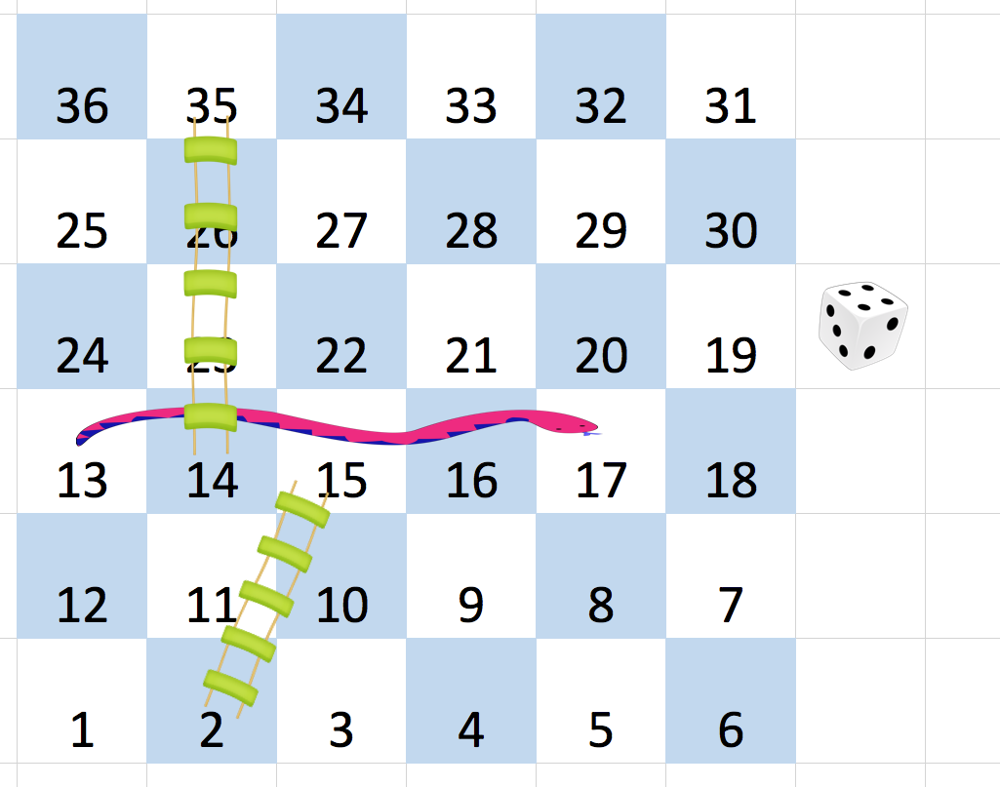
\includegraphics[width=0.4\linewidth]{images/lc0909_example}
	\label{fig:lc0909example}
\end{figure}

\subsection*{Solution}

\section{LC 0841 - Keys and Rooms}
There are {\colorbox{CodeBackground}{\lstinline|n|}} rooms labeled from {\colorbox{CodeBackground}{\lstinline|0|}} to {\colorbox{CodeBackground}{\lstinline|n - 1|}} and all the rooms are locked except for room {\colorbox{CodeBackground}{\lstinline|0|}}. Your goal is to visit all the rooms. However, you cannot enter a locked room without having its key.\\

When you visit a room, you may find a set of distinct keys in it. Each key has a number on it, denoting which room it unlocks, and you can take all of them with you to unlock the other rooms.\\

Given an array {\colorbox{CodeBackground}{\lstinline|rooms|}} where {\colorbox{CodeBackground}{\lstinline|rooms[i]|}} is the set of keys that you can obtain if you visited room {\colorbox{CodeBackground}{\lstinline|i|}}, return {\colorbox{CodeBackground}{\lstinline|true|}} if you can visit all the rooms, or {\colorbox{CodeBackground}{\lstinline|false|}} otherwise.\\

Examples:
\begin{itemize}
	\item {\colorbox{CodeBackground}{\lstinline|rooms = [[1],[2],[3],[]] --> true|}}
	\item {\colorbox{CodeBackground}{\lstinline|rooms = [[1,3],[3,0,1],[2],[0]] --> false|}}
\end{itemize}

\subsection*{Solution}
\begin{lstlisting}
bool canVisitAllRooms(std::vector<std::vector<int>>& rooms) {
	std::stack<int> dfs;                             // Stack to hold keys/rooms to visit.
	dfs.push(0);                                     // Start with room 0.
	std::vector<bool> visited(rooms.size(), false);  // Keep track of visited rooms.
	visited[0] = true;                               // Mark room 0 as visited.
	
	while (!dfs.empty()) {
		int currentRoom = dfs.top();
		dfs.pop();
		for (int key : rooms[currentRoom]) {
			if (!visited[key]) {    // If we haven't visited this room yet.
				visited[key] = true;  // Mark as visited.
				dfs.push(key);        // Add the room to the stack.
			}
		}
	}
	
	// Check if all rooms have been visited.
	for (bool room : visited) {
		if (!room) return false;
	}
	return true;
}
\end{lstlisting}

\section{LC 0847 - Shortest Path Visiting All Nodes}
You have an \ul{undirected, connected graph} of {\colorbox{CodeBackground}{\lstinline|n|}} ({\colorbox{CodeBackground}{\lstinline|n >= 1|}}) nodes labeled from {\colorbox{CodeBackground}{\lstinline|0|}} to {\colorbox{CodeBackground}{\lstinline|n - 1|}}. \\

You are given an array graph where {\colorbox{CodeBackground}{\lstinline|graph[i]|}} is a list of all the nodes connected with node {\colorbox{CodeBackground}{\lstinline|i|}} by an edge.\\

Return the length of the shortest path that visits every node. \\

You may start and stop at any node, you may revisit nodes multiple times, and you may reuse edges.

\begin{itemize}
\item Example 1: {\colorbox{CodeBackground}{\lstinline|graph = [[1,2,3],[0],[0],[0]] --> 4|}}
\begin{figure}[H]
\centering
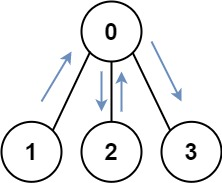
\includegraphics[width=0.18\linewidth]{images/lc0847_eg1}
\label{fig:lc0847eg1}
\end{figure}
One possible path is {\colorbox{CodeBackground}{\lstinline|[1,0,2,0,3]|}}
\item Example 2: {\colorbox{CodeBackground}{\lstinline|graph = [[1],[0,2,4],[1,3,4],[2],[1,2]] --> 4|}}
\begin{figure}[H]
\centering
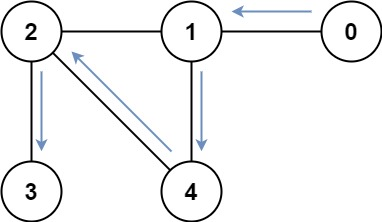
\includegraphics[width=0.3\linewidth]{images/lc0847_eg2}
\label{fig:lc0847eg2}
\end{figure}
One possible path is {\colorbox{CodeBackground}{\lstinline|[0,1,4,2,3]|}}
\end{itemize}

\subsection*{Solution - BFS}
\begin{lstlisting}
int shortestPathLength(std::vector<std::vector<int>>& graph) {
  int n = graph.size();
  std::vector<std::vector<bool>> visited(n, std::vector<bool>(1 << n, false));
  // tuple = {node, visited state, path length}
  std::queue<std::tuple<int, int, int>> q;
  for (int i = 0; i < n; ++i) {
    q.push({i, 1 << i, 1});
    visited[i][1 << i] = true;
  }
  while (!q.empty()) {
    auto [node, state, path_len] = q.front();
    q.pop();
    // all nodes are visited
    if (state == (1 << n) - 1) { return path_len - 1; }
    for (int neighbor : graph[node]) {
      int next_state = state | (1 << neighbor);
      if (!visited[neighbor][next_state]) {
        visited[neighbor][next_state] = true;
        q.push({neighbor, next_state, path_len + 1});
      }
    }
  }
  return -1;
}
\end{lstlisting}

\section{LC 2115 - Find All Possible Recipes from Given Supplies}\label{lc2115}
You have information about {\colorbox{CodeBackground}{\lstinline|n|}} ({\colorbox{CodeBackground}{\lstinline|n >= 1|}}) different recipes, and you are given a string array {\colorbox{CodeBackground}{\lstinline|recipes|}} and a 2D string array {\colorbox{CodeBackground}{\lstinline|ingredients|}}. The {\colorbox{CodeBackground}{\lstinline|i|}}th recipe has the name {\colorbox{CodeBackground}{\lstinline|recipes[i]|}}, and you can create it if you have all the needed ingredients from {\colorbox{CodeBackground}{\lstinline|ingredients[i]|}}. \\

Note that:
\begin{itemize}
\item Ingredients to a recipe may need to be created from other recipes, i.e., {\colorbox{CodeBackground}{\lstinline|ingredients[i]|}} may contain a string that is in {\colorbox{CodeBackground}{\lstinline|recipes|}}.
\item Two recipes may contain each other in their ingredients.
\end{itemize}

You are also given a string array {\colorbox{CodeBackground}{\lstinline|supplies|}} containing all the ingredients that you initially have, and you have an infinite supply of all of them.\\

Return a list of all the recipes that you can create. You may return the answer in any order.\\

\begin{itemize}
\item Example 1:
\begin{lstlisting}
recipes = ["bread"]
ingredients = [["yeast","flour"]]
supplies = ["yeast","flour","corn"]
--> ["bread"]
\end{lstlisting}
We can create "bread" since we have the ingredients "yeast" and "flour".
\item Example 2:
\begin{lstlisting}
recipes = ["bread","sandwich"]
ingredients = [["yeast","flour"],["bread","meat"]]
supplies = ["yeast","flour","meat"]
--> ["bread","sandwich"]
\end{lstlisting}
We can create "bread" since we have the ingredients "yeast" and "flour".\\
We can create "sandwich" since we have the ingredient "meat" and can create the ingredient "bread".
\item Example 3:
\begin{lstlisting}
recipes = ["bread","sandwich","burger"]
ingredients = [["yeast","flour"],["bread","meat"],["sandwich","meat","bread"]]
supplies = ["yeast","flour","meat"]
--> ["bread","sandwich","burger"]
\end{lstlisting}
We can create "bread" since we have the ingredients "yeast" and "flour".\\
We can create "sandwich" since we have the ingredient "meat" and can create the ingredient "bread".\\
We can create "burger" since we have the ingredient "meat" and can create the ingredients "bread" and "sandwich".
\end{itemize}

\section{LC 2101 - Detonate the Maximum Bombs}
You are given a list of bombs. The range of a bomb is defined as the area where its effect can be felt. This area is in the shape of a circle with the center as the location of the bomb.\\

The bombs are represented by a {\colorbox{CodeBackground}{\lstinline|0|}}-indexed 2D integer array {\colorbox{CodeBackground}{\lstinline|bombs|}} where {\colorbox{CodeBackground}{\lstinline|bombs[i] = [x_i, y_i, r_i]|}}. {\colorbox{CodeBackground}{\lstinline|x_i|}} and {\colorbox{CodeBackground}{\lstinline|y_i|}} denote the X-coordinate and Y-coordinate of the location of the {\colorbox{CodeBackground}{\lstinline|i|}}th bomb, whereas {\colorbox{CodeBackground}{\lstinline|r_i|}} denotes the radius of its range.\\

You may choose to detonate a single bomb. When a bomb is detonated, it will detonate all bombs that lie in its range. These bombs will further detonate the bombs that lie in their ranges.\\

Given the list of {\colorbox{CodeBackground}{\lstinline|bombs|}}, return the maximum number of bombs that can be detonated if you are allowed to detonate only one bomb.

\begin{itemize}
\item Example 1: {\colorbox{CodeBackground}{\lstinline|bombs = [[2,1,3],[6,1,4]] --> 2|}}
\begin{figure}[H]
\centering
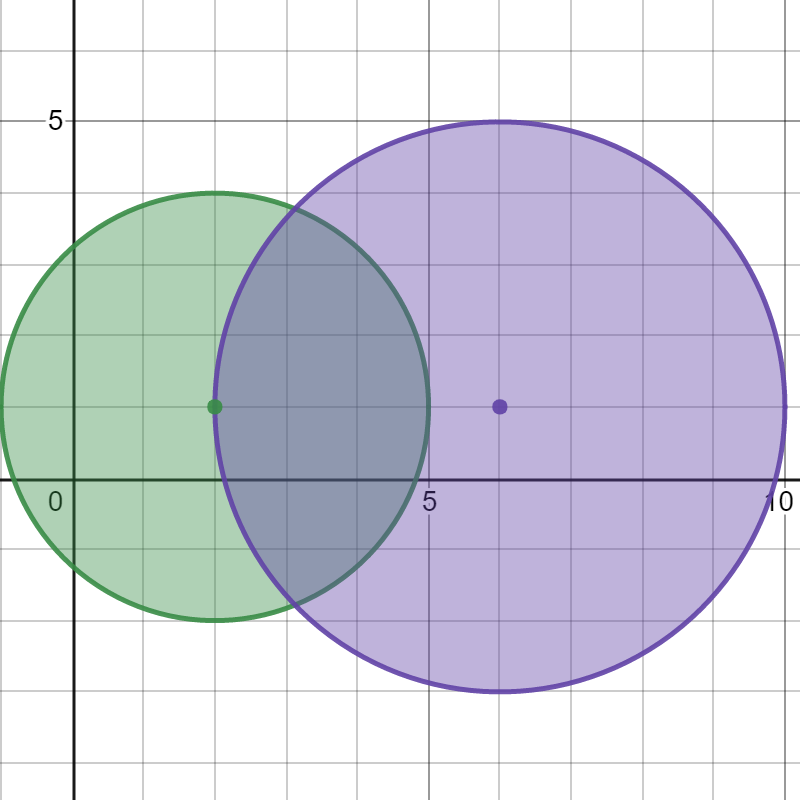
\includegraphics[width=0.3\linewidth]{images/lc2101_eg1}
\end{figure}
The above figure shows the positions and ranges of the {\colorbox{CodeBackground}{\lstinline|2|}} bombs.\\
If we detonate the left bomb, the right bomb will not be affected.\\
But if we detonate the right bomb, both bombs will be detonated.\\
So the maximum bombs that can be detonated is {\colorbox{CodeBackground}{\lstinline|max(1, 2) = 2|}}.
\item Example 2:
\begin{figure}[H]
\centering
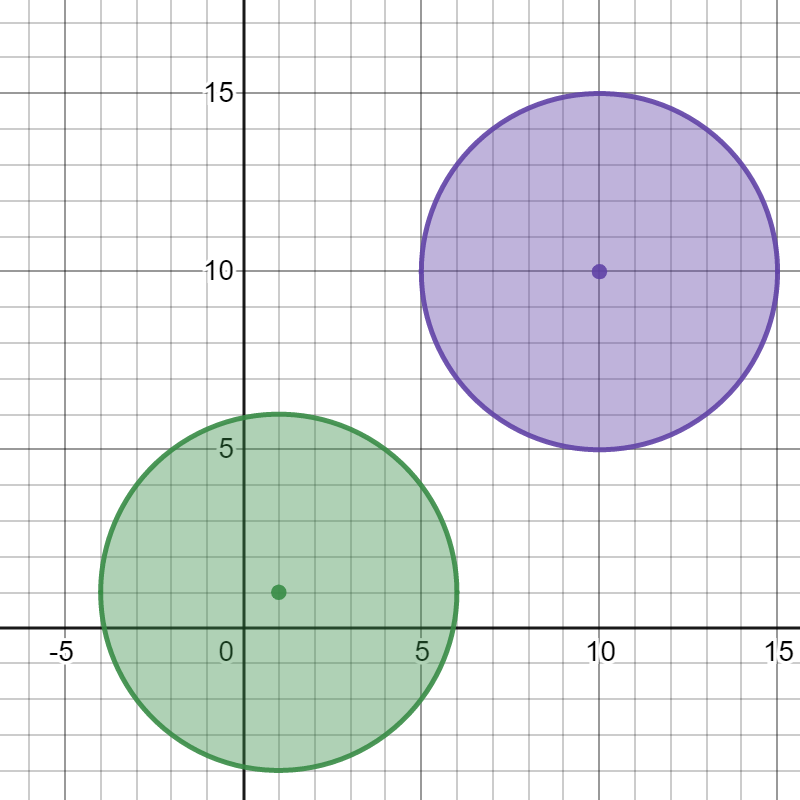
\includegraphics[width=0.3\linewidth]{images/lc2101_eg2}
\end{figure}
Detonating either bomb will not detonate the other bomb, so the maximum number of bombs that can be detonated is {\colorbox{CodeBackground}{\lstinline|1|}}.
\item Example 3:
\begin{figure}[H]
\centering
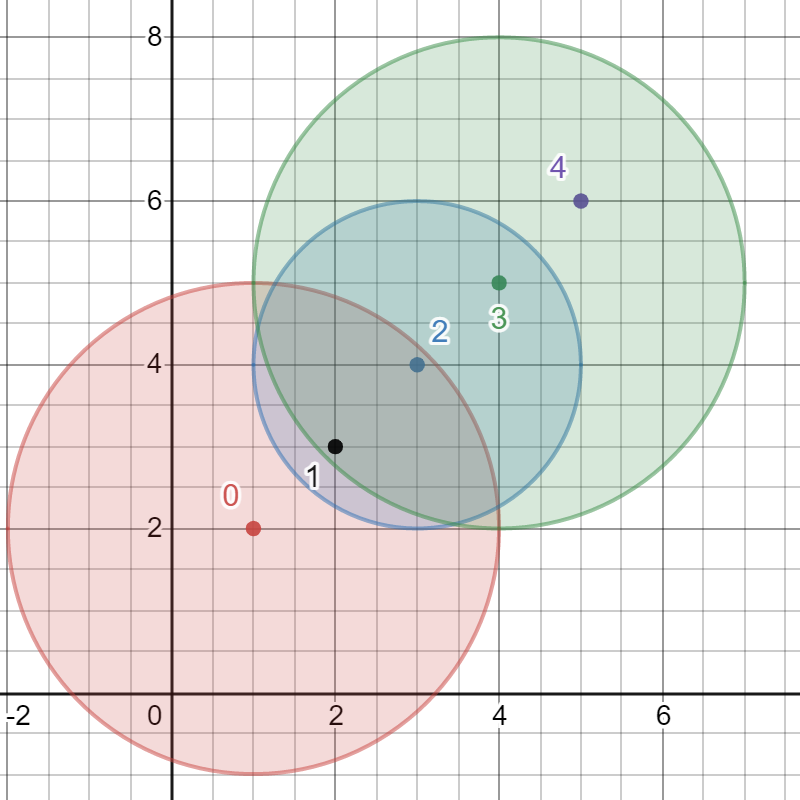
\includegraphics[width=0.3\linewidth]{images/lc2101_eg3}
\end{figure}
The best bomb to detonate is bomb {\colorbox{CodeBackground}{\lstinline|0|}} because:\\
- Bomb {\colorbox{CodeBackground}{\lstinline|0|}} detonates bombs {\colorbox{CodeBackground}{\lstinline|1|}} and {\colorbox{CodeBackground}{\lstinline|2|}}. The red circle denotes the range of bomb {\colorbox{CodeBackground}{\lstinline|0|}}.\\
- Bomb {\colorbox{CodeBackground}{\lstinline|2|}} detonates bomb {\colorbox{CodeBackground}{\lstinline|3|}}. The blue circle denotes the range of bomb {\colorbox{CodeBackground}{\lstinline|2|}}.\\
- Bomb {\colorbox{CodeBackground}{\lstinline|3|}} detonates bomb {\colorbox{CodeBackground}{\lstinline|4|}}. The green circle denotes the range of bomb {\colorbox{CodeBackground}{\lstinline|3|}}.\\
Thus all {\colorbox{CodeBackground}{\lstinline|5|}} bombs are detonated.
\end{itemize}


\section{LC 1584 - Min Cost to Connect All Points}
You are given a \ul{non-empty} array {\colorbox{CodeBackground}{\lstinline|points|}} representing integer coordinates of some points on a 2D-plane, where {\colorbox{CodeBackground}{\lstinline|points[i] = [x_i, y_i]|}}.\\

The cost of connecting two points {\colorbox{CodeBackground}{\lstinline|[xi, yi]|}} and {\colorbox{CodeBackground}{\lstinline|[xj, yj]|}} is the manhattan distance between them: {\colorbox{CodeBackground}{\lstinline|\|x_i - x_j\| + \|y_i - yj_\||}}, where {\colorbox{CodeBackground}{\lstinline|\|val\||}} denotes the absolute value of val.\\

Return the minimum cost to make all points connected. All points are connected if there is exactly one simple path between any two points.

\begin{itemize}
\item {\colorbox{CodeBackground}{\lstinline|points = [[0,0],[2,2],[3,10],[5,2],[7,0]] --> 20|}}
\begin{figure}[H]
\centering
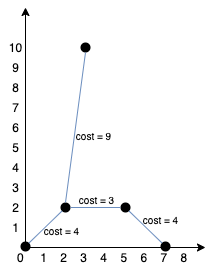
\includegraphics[width=0.25\linewidth]{images/lc1584_eg}
\label{fig:lc1584eg}
\item {\colorbox{CodeBackground}{\lstinline|points = [[3,12],[-2,5],[-4,1]] --> 18|}}
\end{figure}
\end{itemize}

\section{LC 2858 - Minimum Edge Reversals So Every Node Is Reachable}
There is a \ul{simple directed graph} with {\colorbox{CodeBackground}{\lstinline|n|}} nodes labeled from {\colorbox{CodeBackground}{\lstinline|0|}} to {\colorbox{CodeBackground}{\lstinline|n - 1|}}. The graph would form a tree if its edges were bi-directional.\\

You are given an integer {\colorbox{CodeBackground}{\lstinline|n|}} ({\colorbox{CodeBackground}{\lstinline|n >= 2|}}) and a 2D integer array {\colorbox{CodeBackground}{\lstinline|edges|}}, where {\colorbox{CodeBackground}{\lstinline|edges[i] = [u_i, v_i]|}} represents a \ul{directed edge} going from node {\colorbox{CodeBackground}{\lstinline|u_i|}} to node {\colorbox{CodeBackground}{\lstinline|v_i|}}.\\

An edge reversal changes the direction of an edge, i.e., a directed edge going from node {\colorbox{CodeBackground}{\lstinline|u_i|}} to node {\colorbox{CodeBackground}{\lstinline|v_i|}} becomes a directed edge going from node {\colorbox{CodeBackground}{\lstinline|v_i|}} to node {\colorbox{CodeBackground}{\lstinline|u_i|}}.\\

For every node {\colorbox{CodeBackground}{\lstinline|i|}} in the range {\colorbox{CodeBackground}{\lstinline|[0, n - 1]|}}, your task is to independently calculate the minimum number of edge reversals required so it is possible to reach any other node starting from node {\colorbox{CodeBackground}{\lstinline|i|}} through a sequence of directed edges.\\

Return an integer array {\colorbox{CodeBackground}{\lstinline|answer|}}, where {\colorbox{CodeBackground}{\lstinline|answer[i]|}} is the minimum number of edge reversals required so it is possible to reach any other node starting from node {\colorbox{CodeBackground}{\lstinline|i|}} through a sequence of directed edges.

\begin{itemize}
\item Example 1: {\colorbox{CodeBackground}{\lstinline|n = 4, edges = [[2,0],[2,1],[1,3]] --> [1,1,0,2]|}}
\begin{figure}[H]
\centering
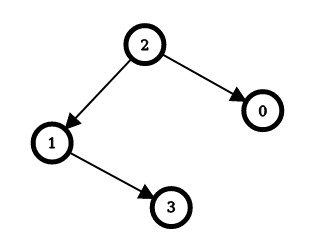
\includegraphics[width=0.3\linewidth]{images/lc2858_eg1}
\label{fig:lc2858eg1}
\end{figure}
The image above shows the graph formed by the edges.\\
For node {\colorbox{CodeBackground}{\lstinline|0|}}: after reversing the edge {\colorbox{CodeBackground}{\lstinline|[2,0]|}}, it is possible to reach any other node starting from node {\colorbox{CodeBackground}{\lstinline|0|}}.\\
So, {\colorbox{CodeBackground}{\lstinline|answer[0] = 1|}}.\\
For node {\colorbox{CodeBackground}{\lstinline|1|}}: after reversing the edge {\colorbox{CodeBackground}{\lstinline|[2,1]|}}, it is possible to reach any other node starting from node {\colorbox{CodeBackground}{\lstinline|1|}}.\\
So, {\colorbox{CodeBackground}{\lstinline|answer[1] = 1|}}.\\
For node {\colorbox{CodeBackground}{\lstinline|2|}}: it is already possible to reach any other node starting from node {\colorbox{CodeBackground}{\lstinline|2|}}.\\
So, {\colorbox{CodeBackground}{\lstinline|answer[2] = 0|}}.\\
For node {\colorbox{CodeBackground}{\lstinline|3|}}: after reversing the edges {\colorbox{CodeBackground}{\lstinline|[1,3]|}} and {\colorbox{CodeBackground}{\lstinline|[2,1]|}}, it is possible to reach any other node starting from node {\colorbox{CodeBackground}{\lstinline|3|}}.\\
So, {\colorbox{CodeBackground}{\lstinline|answer[3] = 2|}}.
\item Example 2: {\colorbox{CodeBackground}{\lstinline|n = 3, edges = [[1,2],[2,0]] --> [2,0,1]|}}
\begin{figure}[H]
\centering
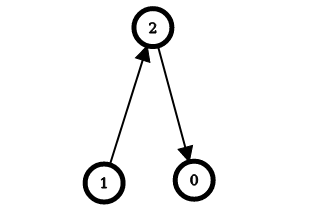
\includegraphics[width=0.3\linewidth]{images/lc2858_eg2}
\label{fig:lc2858eg2}
\end{figure}
The image above shows the graph formed by the edges.\\
For node {\colorbox{CodeBackground}{\lstinline|0|}}: after reversing the edges {\colorbox{CodeBackground}{\lstinline|[2,0]|}} and {\colorbox{CodeBackground}{\lstinline|[1,2]|}}, it is possible to reach any other node starting from node {\colorbox{CodeBackground}{\lstinline|0|}}.\\
So, {\colorbox{CodeBackground}{\lstinline|answer[0] = 2|}}.\\
For node {\colorbox{CodeBackground}{\lstinline|1|}}: it is already possible to reach any other node starting from node {\colorbox{CodeBackground}{\lstinline|1|}}.\\
So, {\colorbox{CodeBackground}{\lstinline|answer[1] = 0|}}.\\
For node {\colorbox{CodeBackground}{\lstinline|2|}}: after reversing the edge {\colorbox{CodeBackground}{\lstinline|[1, 2]|}}, it is possible to reach any other node starting from node {\colorbox{CodeBackground}{\lstinline|2|}}.\\
So, {\colorbox{CodeBackground}{\lstinline|answer[2] = 1|}}.
\end{itemize}

\section{LC 0547 - Number of Provinces}
There are {\colorbox{CodeBackground}{\lstinline|n|}} ({\colorbox{CodeBackground}{\lstinline|n >= 1|}}) cities. Some of them are connected, while some are not. If city {\colorbox{CodeBackground}{\lstinline|a|}} is connected directly with city {\colorbox{CodeBackground}{\lstinline|b|}}, and city {\colorbox{CodeBackground}{\lstinline|b|}} is connected directly with city {\colorbox{CodeBackground}{\lstinline|c|}}, then city {\colorbox{CodeBackground}{\lstinline|a|}} is connected indirectly with city {\colorbox{CodeBackground}{\lstinline|c|}}.\\

A \ul{province} is a group of directly or indirectly connected cities and no other cities outside of the group.\\

You are given an {\colorbox{CodeBackground}{\lstinline|n x n|}} matrix {\colorbox{CodeBackground}{\lstinline|isConnected|}} where {\colorbox{CodeBackground}{\lstinline|isConnected[i][j] = 1|}} if the {\colorbox{CodeBackground}{\lstinline|i|}}th city and the {\colorbox{CodeBackground}{\lstinline|j|}}th city are directly connected, and {\colorbox{CodeBackground}{\lstinline|isConnected[i][j] = 0|}} otherwise. Note that {\colorbox{CodeBackground}{\lstinline|isConnected[i][j] == isConnected[j][i]|}}.

Return the total number of provinces.

\begin{itemize}
\item {\colorbox{CodeBackground}{\lstinline|isConnected = [[1,1,0],[1,1,0],[0,0,1]] --> 2|}}
\begin{figure}[H]
\centering
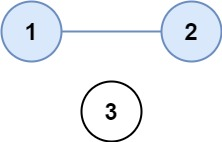
\includegraphics[width=0.15\linewidth]{images/lc0547_eg1}
\end{figure}
\item {\colorbox{CodeBackground}{\lstinline|isConnected = [[1,0,0],[0,1,0],[0,0,1]] --> 3|}}
\begin{figure}[H]
\centering
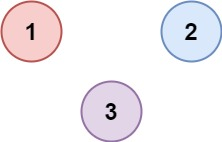
\includegraphics[width=0.15\linewidth]{images/lc0547_eg2}
\end{figure}
\end{itemize}

\section{LC 0797 - All Paths From Source to Target}
Given a \ul{directed acyclic graph (DAG)} of {\colorbox{CodeBackground}{\lstinline|n|}} ({\colorbox{CodeBackground}{\lstinline|n >= 2|}}) nodes labeled from {\colorbox{CodeBackground}{\lstinline|0|}} to {\colorbox{CodeBackground}{\lstinline|n - 1|}}, find all possible paths from node {\colorbox{CodeBackground}{\lstinline|0|}} to node {\colorbox{CodeBackground}{\lstinline|n - 1|}} and return them in any order.\\

The graph is given as follows: {\colorbox{CodeBackground}{\lstinline|graph[i]|}} is a list of all nodes you can visit from node {\colorbox{CodeBackground}{\lstinline|i|}} (i.e., there is a directed edge from node {\colorbox{CodeBackground}{\lstinline|i|}} to node {\colorbox{CodeBackground}{\lstinline|graph[i][j]|}}).

\begin{itemize}
\item {\colorbox{CodeBackground}{\lstinline|graph = [[1,2],[3],[3],[]] --> [[0,1,3],[0,2,3]]|}}
\begin{figure}[H]
\centering
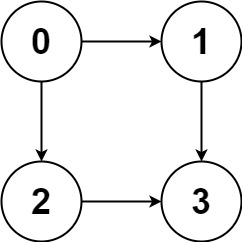
\includegraphics[width=0.15\linewidth]{images/lc0797_eg1}
\end{figure}
\item {\colorbox{CodeBackground}{\lstinline|graph = [[4,3,1],[3,2,4],[3],[4],[]] --> [[0,4],[0,3,4],[0,1,3,4],[0,1,2,3,4],[0,1,4]]|}}
\begin{figure}[H]
\centering
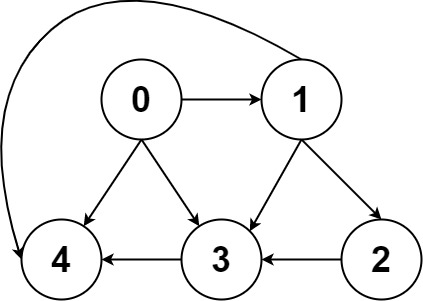
\includegraphics[width=0.28\linewidth]{images/lc0797_eg2}
\end{figure}
\end{itemize}